% Chapter Template

\chapter{Background} % Main chapter title

\label{chp:background} % Change X to a consecutive number; for referencing this chapter elsewhere, use \ref{ChapterX}

This chapter includes required background to understand the thesis proposal presented in the following chapters.

\section{Convolutional Neural Networks (CNN)}
CNN is initially introduced by LeCun \cite{lecun1989handwritten} which is based on learning adaptive convolutional kernels. CNN consist of two parts convbase and densebase parts. For the Convbase instead of connecting all of the units in a layer to all the units in a preceding layer, convolutional networks organize each layer into feature maps \cite{lecun1989handwritten}, which
can be though of as parallel planes or channels. In a convolutional layer, the weighted sums are only performed within a small local window \textit{i.e)} receptive field, and weights are identical for all pixels, just as in regular shift-invariant image convolution and correlation. This parameter sharing reduce the required total number of parameter and allows learning shift invariant convolutional kernels. These convolutional kernels produce equivariant features maps. Fig. \ref{lenet} represents typical CNN architecture of LeNet.
\begin{figure}
    \begin{center}
        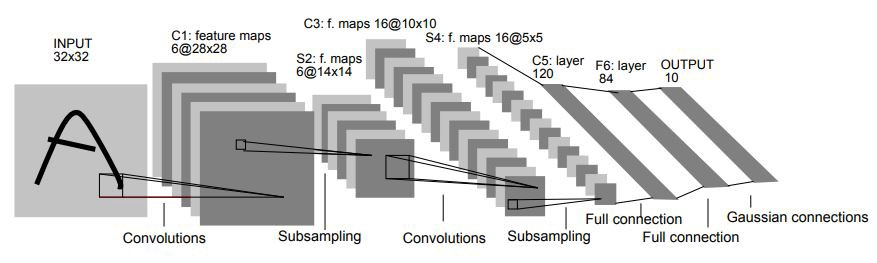
\includegraphics[width=\textwidth]{Figures/LeNetCNN.jpeg}
        \caption{Typical CNN architecture}
        \label{lenet}
    \end{center}
\end{figure}
\subsection{Convolutional Layer}
The building block of the convolutional layer is the 2D convolutional kernel. Fig. \ref{conv2Dlayer} illustrates the 2D convolutional layer. Each 2D convolution kernel takes as input all of the $C_{i-1}$ channels in the preceding layer, windowed to a small area, and produces the values in one of the $C_{i}$ channels in the next layer. For each of the output channels, we have $K^2\times C_{i-1}$ kernel weights, so the total number of learnable parameters in each convolutional layer is $K^2\times C_{i-1} \times C_{i}$. In Fig. \ref{conv2Dlayer}, we have $C_{i-1} = 6$ input channels and $C_{i} = 4$ output channels, with an $K = 3$ convolution window, for a total of $9 \times 6 \times 4$ learnable weights, shown in the middle column of the figure. Since the convolution is applied at each of the $W \times H$ pixels in a given layer, the amount of computation (multiply-adds) in each forward and backward pass
over one sample in a given layer is $W\times H \times K^{2} \times C_{i-1} \times C_{i}$.
To fully determine the behavior of a convolutional layer, we still need to specify the following hyperparameter:
\begin{itemize}
    \item \textbf{Padding.} Padding is used to preserve the spatial dimension of the input feature map after the convolution operation is performed. Typically, it is performed by inserting $\lfloor K/2 \rfloor$ columns for both sides and $\lfloor K/2 \rfloor$ rows to the top and bottom.
    \item \textbf{Stride.} Stride is the step taken between two centers when performing the convolution operation. Typically, Stride is equal to $1$. Stride can act as down sampling operation that can be performed instead of the pooling operation.
    \item Dilation.
    \item Grouping.
\end{itemize}





\begin{figure}
    \begin{center}
        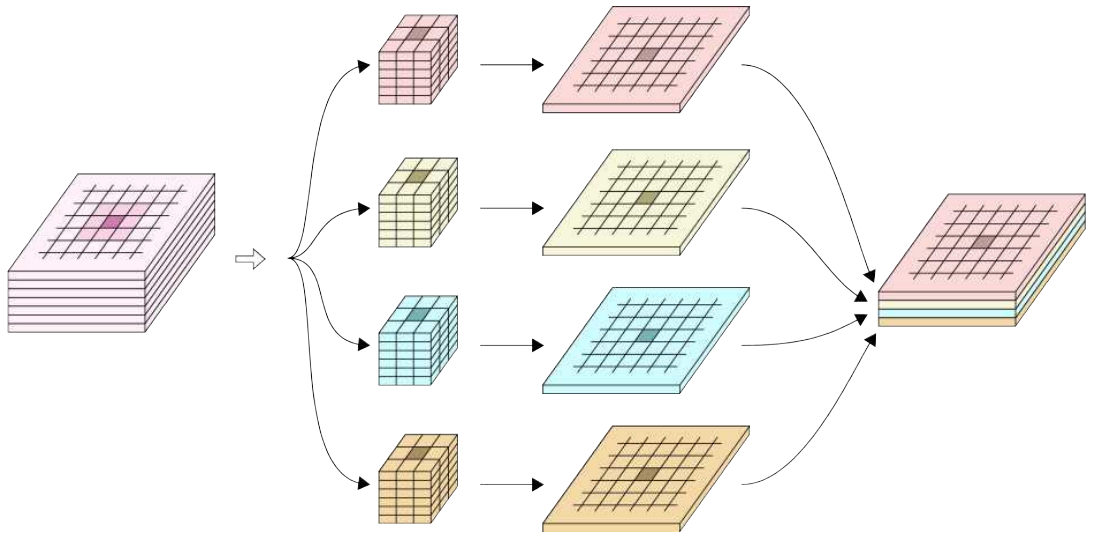
\includegraphics[width=\textwidth]{Figures/2DConvKernels.png}
        \caption{Convolutional layer with single input feature map and four convolutional kernels}
        \label{conv2Dlayer}
    \end{center}
\end{figure}


Batch normalization algorithm is described as follows:

\vspace*{1.3\baselineskip}
\begin{algorithmic}[1]

\REQUIRE : Minibatch activation values $x$ : $\mathcal B = \{x_{1,\ldots,m}\}$ ; parameters to be learned $\gamma$ ,$\beta$.

\ENSURE  : $\{y_i = \mathrm{BN}_{\gamma,\beta}(x_i)\}$
\vspace*{.7\baselineskip}
\STATE $\mu_{\mathcal B} \leftarrow \frac1m \sum_{i = 1}^m x_i$
\vspace*{.7\baselineskip}
\STATE $\sigma^2_{\mathcal B} \leftarrow \frac1m \sum_{i=1}^m (x_i - \mu_{\mathcal B})^2$
\vspace*{.7\baselineskip}
\STATE $\hat x_i \leftarrow \frac{x_i - \mu_{\mathcal B}}{\sqrt{\sigma_{\mathcal B}^2 + \epsilon}}$
\vspace*{.7\baselineskip}
\STATE $y_i \leftarrow \gamma \hat x_i + \beta \equiv \mathrm{BN}_{\gamma,\beta}(x_i)$

\end{algorithmic}